\section{Displaced photon gun}
\label{sec:gun}

To measure the dependence of reconstruction performance on displacement, we
need samples in which the shower energy and trajectory can be controlled
independently of a particular LLP model. For this purpose, Bruno Alves developed
the original displaced-particle gun for the project (CMSSW pull request
\href{https://github.com/cms-sw/cmssw/pull/51006}{\#51006}). My contribution was
to test and improve this generator: I revised its sampling and
configuration, corrected the production timing, and updated the beamspot choice
in the generation workflow. These improvements are collected in pull request
\href{https://github.com/cms-sw/cmssw/pull/51489}{\#51489}.

The studies use photons, whose trajectories are not bent by the magnetic field.
The photons are inserted into the simulation immediately before HGCAL, so they
do not traverse the tracker and convert or shower there. This isolates the response to calorimeter for a non-pointing photon. The gun therefore supplies a
controlled test of the reconstruction geometry; it does not simulate the full
production and decay of an LLP.

\subsection{Trajectory geometry and surface constraints}

The construction distinguishes the \emph{sampled origin} from the actual
\emph{production vertex} passed to the detector simulation. The origin is a
point in the plane $z=0$,
\begin{equation}
  \mathbf{x}_0=(\R\cos\phi_0,\R\sin\phi_0,0),
\end{equation}
so its radius is exactly the displacement observable defined in
Section~\ref{sec:displacement}. Given a momentum polar angle $\theta$ and
azimuth $\phi_p$, the straight trajectory is
\begin{equation}
  \mathbf{x}_{\perp}(z)=\mathbf{x}_{0,\perp}
    +z\tan\theta\,(\cos\phi_p,\sin\phi_p).
  \label{eq:gunline}
\end{equation}
Here $\theta$ is measured from the positive beam axis, while $\phi_0$ specifies
the position of the origin and $\phi_p$ specifies the momentum direction. These
two azimuths do not need to coincide. The non-pointing angle $\alphainc$ follows from
the resulting trajectory and impact point; it is not independently sampled.

The photon is created where this line crosses a configurable
\emph{production plane}, placed at $z=\SI{319}{cm}$ in the example
configuration. Its position must lie within a specified annulus, optionally
restricted in azimuth. An additional \emph{target plane}, near the back of the
electromagnetic calorimeter at $z\simeq\SI{362}{cm}$, can impose a second
annular acceptance. Requiring the line to pass through both regions selects
trajectories that enter the calorimeter and continue through its volume. Suitable radial margins can reduce edge leakage, although an accepted
trajectory alone does not guarantee containment of the entire shower, whose
transverse spread is set by the calorimeter's Moli\`ere radius. The
target constraint is optional and assumes straight propagation, so the
implementation permits it only for neutral particles.

In particular, neither surface is a second independently sampled vertex. Both
constrain the same line from $\mathbf{x}_0$, and the production vertex is
obtained by evaluating Eq.~\eqref{eq:gunline} at the production-plane position.
Consequently, back-extrapolating the generated momentum from that vertex
recovers the sampled $\R$, even though the photon is actually introduced into
the simulation far downstream of $z=0$.

\subsection{Sampling without biasing the displacement scan}

The improved gun supports two distributions for the origin radius. Sampling
$\R^2$ uniformly gives a constant density per unit transverse area, with
$\mathrm{d}N/\mathrm{d}\R\propto\R$. Sampling $\R$ uniformly instead gives
equal expected populations in equal-width displacement bins. We use the latter
for displacement scans. The origin azimuth is sampled uniformly within its
configured range.

A simple approach would draw a direction and discard the entire trial whenever
it misses either surface. This can be inefficient and, if the origin is also
redrawn, changes the accepted displacement distribution according to the
geometric acceptance. The improved implementation holds the sampled origin fixed
and constructs the allowed polar-angle intervals before drawing $\theta$.
For a trial momentum azimuth $\phi_p$, write $s=\tan\theta$. At a surface
$z=z_k$, the squared transverse radius is
\begin{equation}
  r_k^2(s)=\R^2+2z_k\R\cos(\phi_p-\phi_0)s+z_k^2s^2.
  \label{eq:gunconstraint}
\end{equation}
The annular requirement
$r_{k,\min}^2\leq r_k^2(s)\leq r_{k,\max}^2$ gives allowed intervals in
$s$. The gun intersects these intervals for the production plane, the optional
target plane, and the configured $\theta$ bounds. It then samples uniformly in
$\theta$ over the surviving intervals, weighting each interval by its angular
width.

Momentum azimuths with no allowed interval are retried. Spatial azimuthal cuts
on the surfaces are checked after sampling and can also reject a direction.
The origin remains fixed throughout: exhausting the configurable attempt limit
raises an error instead of silently replacing an inconvenient origin. Geometry
checks also reject some incompatible configurations before generation begins.
This preserves the requested origin distribution in a successfully generated
sample while avoiding many impossible direction trials. It does not imply that
the accepted impact positions or the overall $\theta$ distribution are uniform;
both reflect the surface constraints.

The momentum magnitude is sampled after a valid trajectory has been found. The
configuration explicitly selects either a uniform total-energy distribution or
a uniform transverse-momentum distribution, together with the corresponding
range. For photons these choices are related by
\begin{equation}
  E=\frac{p_T}{\sin\theta},
  \label{eq:gunenergy}
\end{equation}
in units with $c=1$. Thus, a fixed $p_T$ range produces increasingly energetic
photons at small $\theta$. Sampling $E$ directly allows the energy distribution
to be held independent of the accepted direction, which is useful when
isolating displacement effects.

\begin{figure*}[!tp]
  \centering
  \begin{subfigure}[t]{0.49\textwidth}
    \centering
    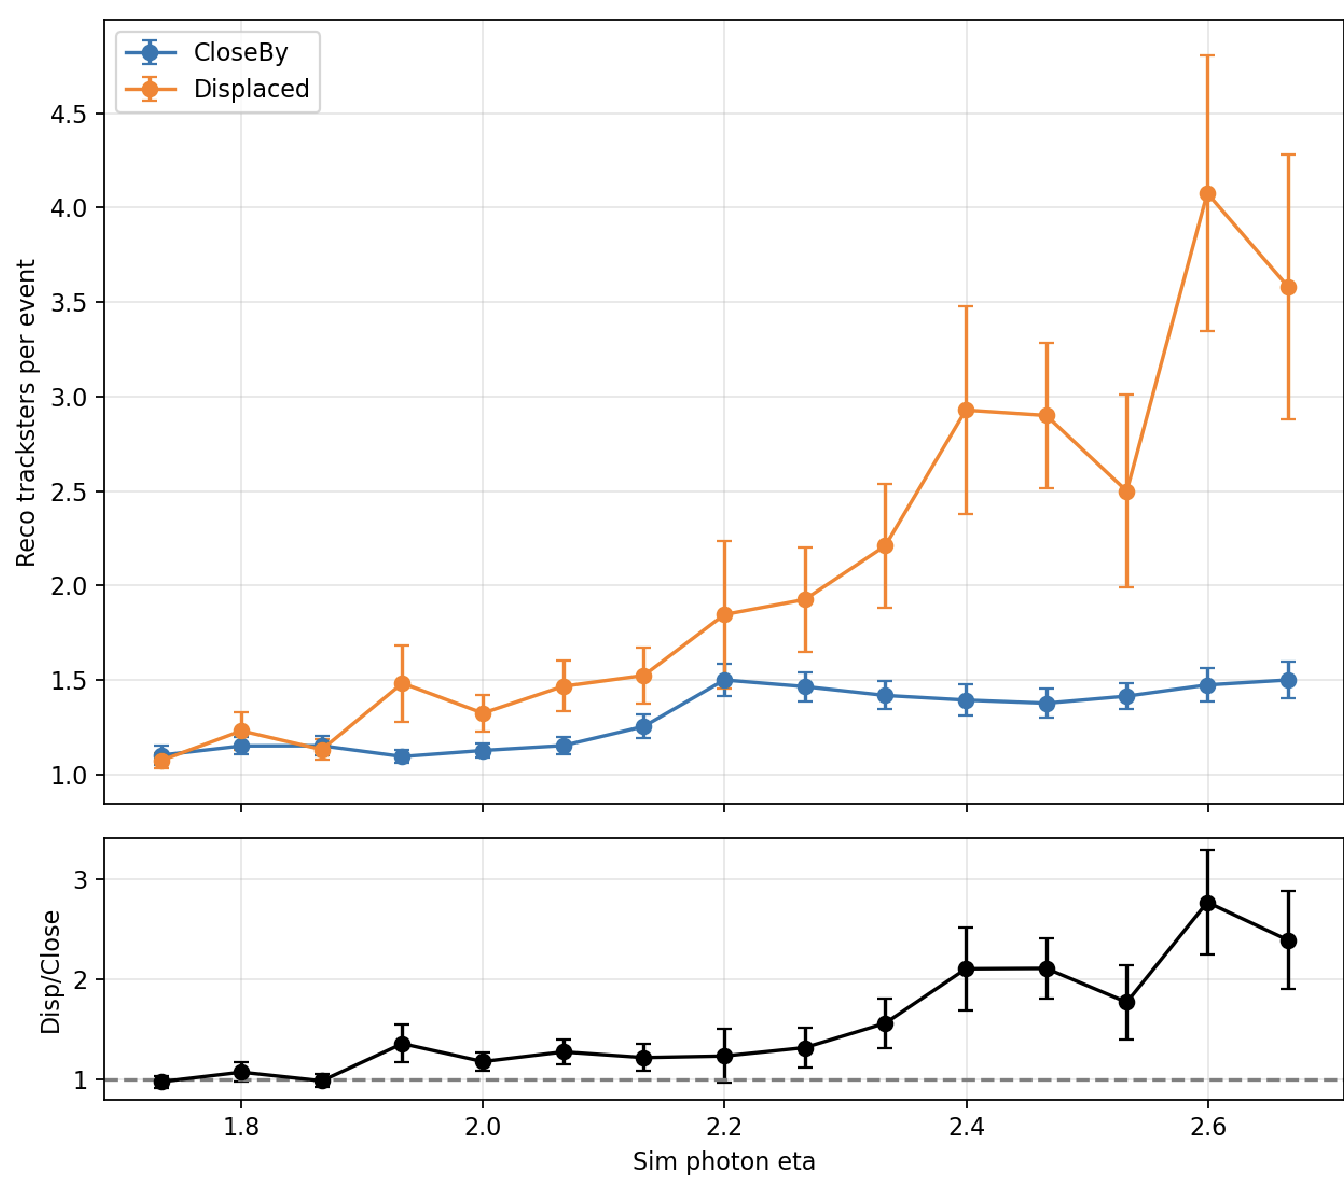
\includegraphics[width=\linewidth]{figures/gun_comparison_pt.png}
    \caption{Displaced gun sampling $p_T$}
  \end{subfigure}
  \hfill
  \begin{subfigure}[t]{0.49\textwidth}
    \centering
    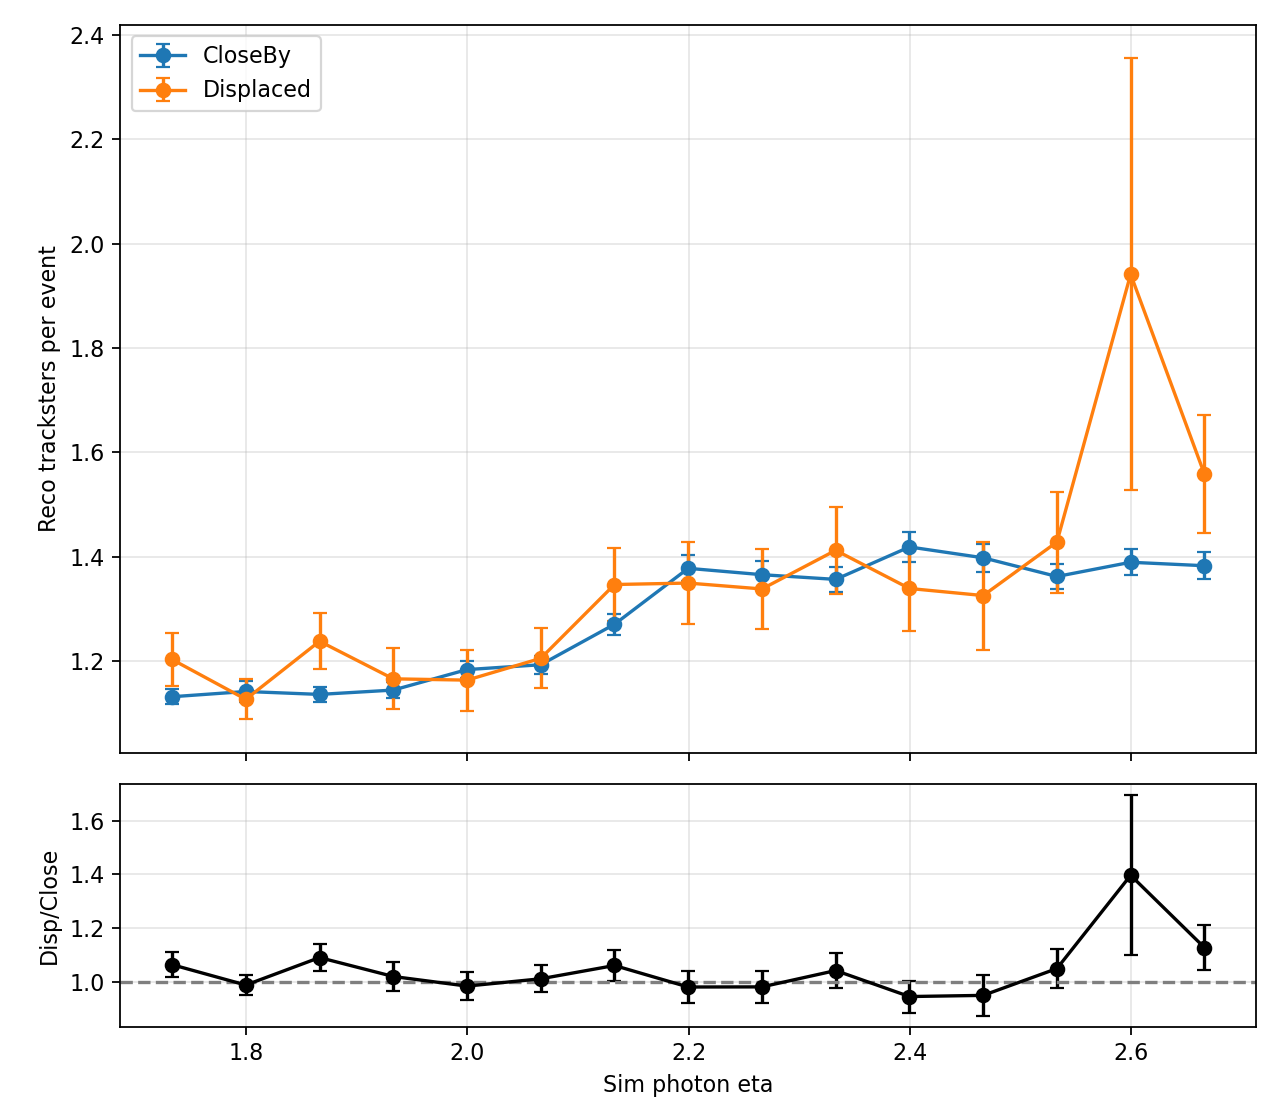
\includegraphics[width=\linewidth]{figures/gun_comparison_energy.png}
    \caption{Displaced gun sampling energy}
  \end{subfigure}
  \caption{Pointing-control comparison of the CloseBy and displaced guns. The upper panels show the mean number of
  reconstructed Tracksters per event versus simulated-photon pseudorapidity;
  each event contains one generated photon, so ideal reconstruction would give
  a multiplicity of one. Values above one indicate shower fragmentation.
  The lower panels show the displaced-to-CloseBy ratio. These plots
  compare the energy-sampling choices, rather than the timing correction.}
  \label{fig:guncomparison}
\end{figure*}

\subsection{Timing and validation of the pointing control}

Before interpreting displaced-shower failures, we tested the pointing limit
$\R=0$ against the existing CloseBy gun. Each event contains a single generated
photon, so ideally its shower would be reconstructed as exactly one Trackster;
a larger multiplicity signals fragmentation of that shower. At $\R=0$ the
displaced gun generates pointing trajectories and should reproduce the CloseBy
response when the kinematics and generation conditions are matched. Instead,
it initially produced substantially more Tracksters per event than CloseBy,
revealing excessive fragmentation even before any displacement was introduced.
Investigating this discrepancy exposed problems in the sample setup.

The first was the production time. The original gun assigned $t=0$ to a photon
created immediately before HGCAL, ignoring the flight time required to reach
that point. Its signals therefore arrived earlier than a particle travelling
at the speed of light from the interaction point could have reached the
calorimeter. Such arrival times are incompatible with the timing assumptions
of the hit-reconstruction chain, which rejected affected signals. The resulting
reconstructed energy was both severely reduced and unevenly retained across
the shower. This disrupted the energy deposits available for clustering,
breaking a single photon shower into several reconstructed Tracksters and
inflating the multiplicity. It was therefore a consequence of the
incorrect generation time, rather than evidence of a displacement-induced
clustering failure at $\R=0$.
The corrected implementation assigns a time from the path length and particle
velocity. More precisely, its present convention is
\begin{equation}
  ct_{\mathrm{prod}}=|\mathbf{x}_0|
       +\frac{|\mathbf{x}_{\mathrm{prod}}-\mathbf{x}_0|}{\beta},
  \qquad \beta=\frac{|\mathbf{p}|}{E},
  \label{eq:guntime}
\end{equation}
where the expression for $\beta$ uses $c=1$. The first segment, from the nominal
interaction point to the sampled origin, is assumed to be traversed at the
speed of light; the second uses the generated particle's velocity. For photons,
$\beta=1$. This is a prescribed timing convention rather than a sampled LLP
lifetime. At $\R=0$ it reduces to the ordinary photon flight time to the
production plane, about $\SI{11}{ns}$ for these geometries. Correcting the time
partially removed the anomalous behaviour of the pointing control.

A second difference was the sampled momentum variable. The displaced gun used
$p_T$ sampling, whereas the CloseBy reference sampled energy. By
Eq.~\eqref{eq:gunenergy}, the former generated much higher energies at large
pseudorapidity, where the showers split into more Tracksters. Introducing direct
energy sampling removed most of the remaining multiplicity discrepancy
(Fig.~\ref{fig:guncomparison}). Agreement is close over most of the displayed
range, with some differences in the highest-$\eta$ bins; the comparison
does not establish exact equivalence of the two samples.

Finally, the displaced-particle workflow used the
\texttt{DBrealisticHLLHC} beamspot smearing, which moved the carefully placed
production vertices and affected the truth-particle selection near the HGCAL
boundary. The workflow was changed to the \texttt{CloseBy} beamspot prescription
appropriate to particles generated at the calorimeter. Together, the timing,
energy-sampling and beamspot corrections established a usable pointing
reference for the displacement scans that follow.
